\section{Coupling Hydrodynamics with Gravity in the Evolution Model}

I utilize the Astrophysical Multi-purpose Software Environment (AMUSE, \cite{pelupessy2013astrophysical,portegies2018astrophysical}), a comprehensive computational tool, to accurately simulate and solve for these physical processes in a self-consistent manner.  The software is written in Python and allows users to combine multiple astrophysical codes into a single simulation. 

The key feature of AMUSE is the Bridge method, first introduced by \cite{fujii2007bridge} and used to combine two different gravity solvers. The coupled integrator divides the Hamiltonian of the combined solution and iteratively integrates it with robust numerical integration techniques. As a result, the method can be implemented in general when the dynamics of a system can be divided into multiple regimes \citep{zwart2013multi}. In this section, I focus on coupling gravity and hydrodynamics which is the focus of this work.
\begin{figure}[H]
    \centering
    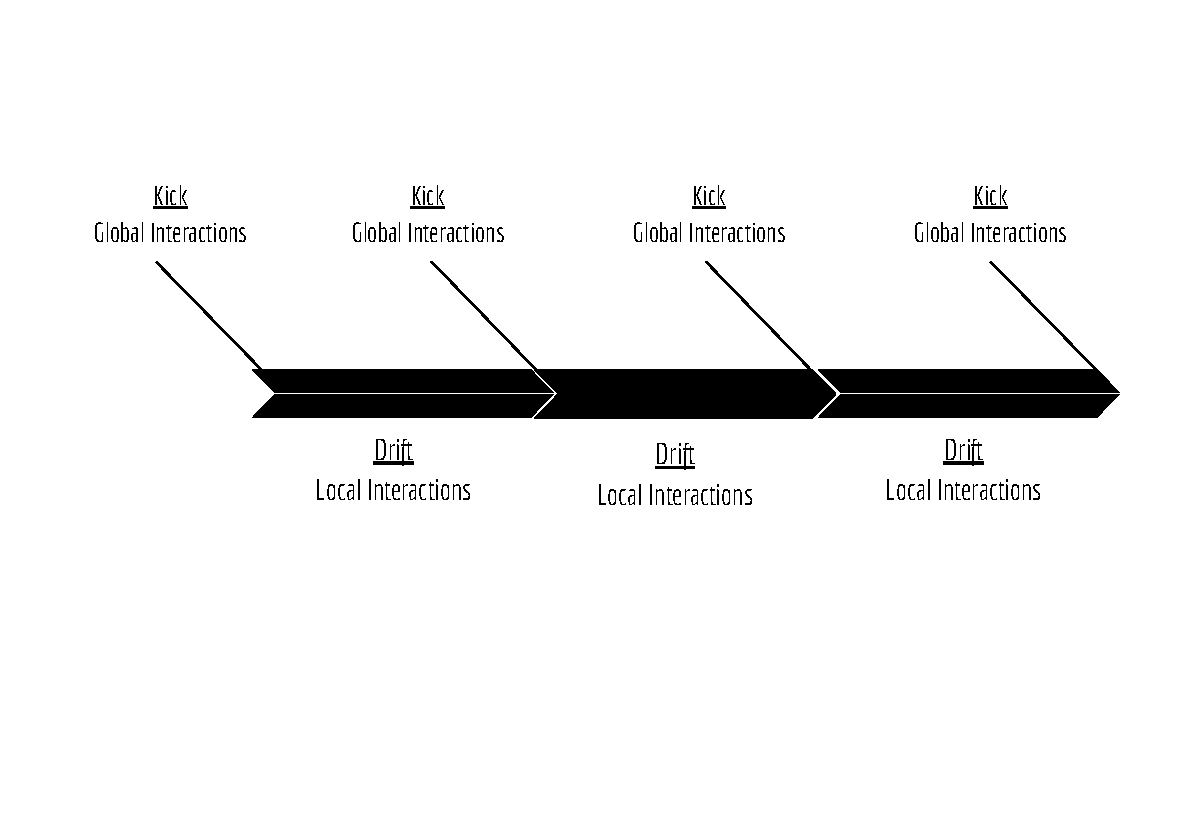
\includegraphics[width=0.9\textwidth]{Thesis/figures/kick_drift_kick.pdf}
    \caption{Schematic kick–drift–kick procedure.}
    \label{fig:kick_drift_kick}
\end{figure}
\cite{saitoh2010fast} showed that the dynamical equations for SPH evolution can be derived from a Hamiltonian formalism, hence the Bridge formalism is applicable to a separation of purely gravitational and SPH particles. In my case, GADGET2 (see \cref{sub:gadget2}) handles the self-gravity and hydrodynamics of the gas, while Huayano (see \cref{sub:huayano}) the gravitational dynamics of the inner binary. Using the Bridge method I achieve a second-order coupling between gravitational dynamics and hydrodynamics. As a result, the hydrodynamical solver is affected by the gravitational potential of its own particles as well as the gravitational potential of the inner binary. Furthermore, the hydrodynamics, namely gas drag, impacts the orbits of the two inner stars.

The evolution via the Bridge method can be implemented as a kick–drift–kick scheme, as illustrated in \cref{fig:kick_drift_kick}. More specifically:
\begin{enumerate}
    \item Kick (Inner Binary, Huayano): Initially, Huayano is used to calculate the gravitational forces operating on the inner binary. These forces "kick" the point masses, causing them to change velocity.
    \item Drift (Inner Binary, Huayano): With the revised velocities of the point masses, Huayano is used to evolve their positions forward in time, assuming a constant velocity over a short time period.
    \item Kick (Tertiary, GADGET2): At this point, Bridge is used to transmit the modified positions and velocities of the point masses from Huayano to GADGET2. The latter utilizes these positions to determine the gravitational forces exerted by the point masses on the 3D hydrodynamical model. These forces "kick" the SPH particles and the core particle, causing their velocities to change.
    \item Drift (Tertiary, GADGET2): Now, using the updated velocities of the 3D hydrodynamical model, GADGET2 evolves the particles positions forward in time allowing for fluid flow and interactions based on the combined effects of gravity and hydrodynamics.
    \item Kick (again) (Inner Binary, Huayano): Once again, Bridge is used, to transport the new positions and velocities of the 3D hydrodynamical model from GADGET2 back to Huayano. Huayano recalculates the gravitational forces acting on the point masses by the 3D hydrodynamical model. These forces "kick" the point masses once more, causing their velocities to change.
    \item Drift (again) (Inner Binary, Huayano): Finally, with the updated velocities of the point masses, Huayano is used to evolve their positions forward in time again, assuming a constant velocity over a short time period.
\end{enumerate}

Each code operates on their own internal time steps, while the Bridge time step  defines the time interval at which the codes interact with each other. Hence, its an important parameter to 
accurately model the coupling between hydrodynamics and gravity. Nevertheless, a time step, $t_{bridge}$, which is about a fraction of $1/64$ the inner binary orbital period, see \cref{tab:system_orbit_param}, provides converged solutions. 

A schematic representation of the entire process is provided in \cref{fig:schematic_method}

\begin{figure}[htp]
    \centering
    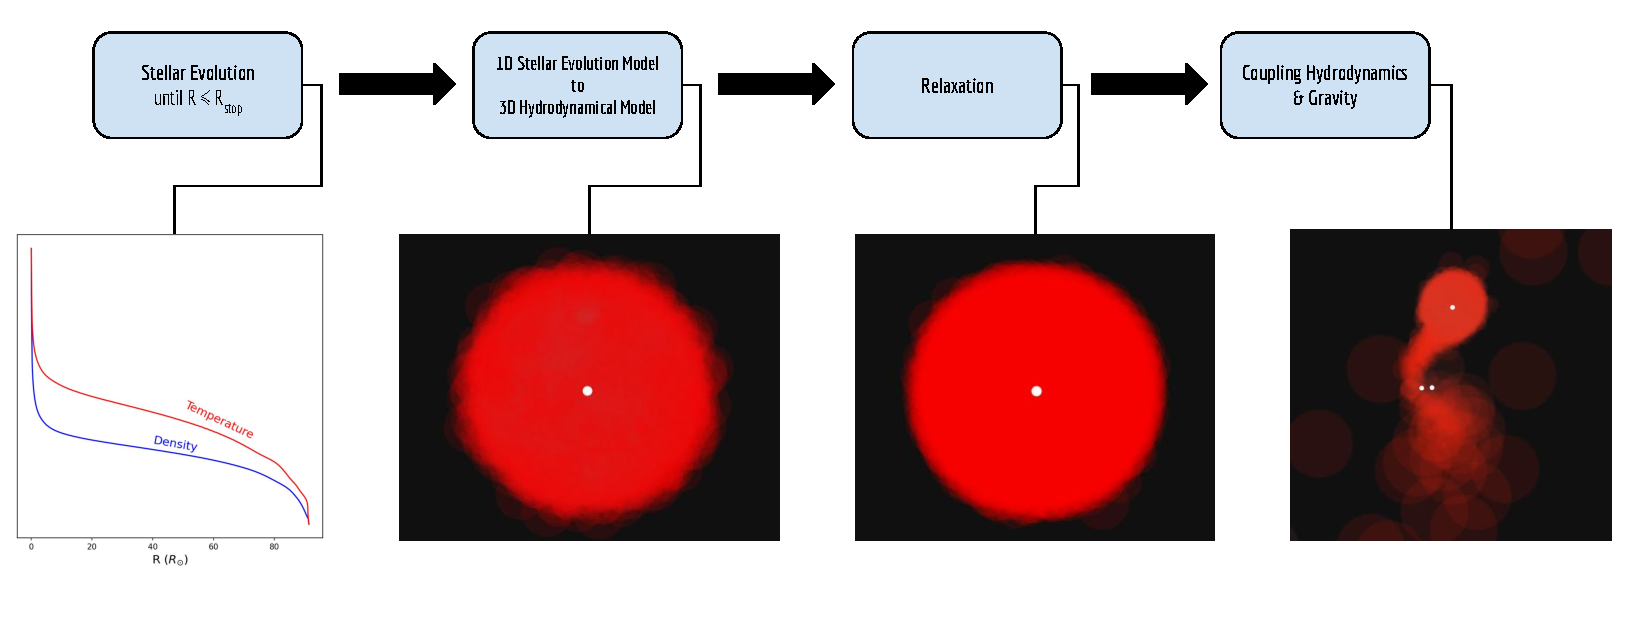
\includegraphics[width=\textwidth]{Thesis/graphs/method_schematic.pdf}
    \caption{Schematic representation of the steps taken to simulate mass transfer in the triple system with a Roche-lobe filling outer star. The white points are the purely gravitational particles representing the core and the inner binary components. The red points are the SPH particles representing the gas having an adaptive smoothing length.}
    \label{fig:schematic_method}
\end{figure}



